\documentclass{article} % For LaTeX2e
\usepackage{nips14submit_e,times}
\usepackage{amsmath}
\usepackage{amsthm}
\usepackage{amssymb}
\usepackage{mathtools}
\usepackage{hyperref}
\usepackage{url}
\usepackage{algorithm}
\usepackage[noend]{algpseudocode}
%\documentstyle[nips14submit_09,times,art10]{article} % For LaTeX 2.09

\usepackage{mathrsfs}
\usepackage{graphicx}
\usepackage{caption}
\usepackage{subcaption}

\def\eQb#1\eQe{\begin{eqnarray*}#1\end{eqnarray*}}
\def\aB#1\aE{\begin{align*}#1\end{align*}}
\def\eQnb#1\eQne{\begin{align}#1\end{align}}
\providecommand{\e}[1]{\ensuremath{\times 10^{#1}}}
\providecommand{\pb}[0]{\pagebreak}

\newcommand{\E}{\mathrm{E}}
\newcommand{\Var}{\mathrm{Var}}
\newcommand{\Cov}{\mathrm{Cov}}

\def\Qb#1\Qe{\begin{question}#1\end{question}}
\def\Sb#1\Se{\begin{solution}#1\end{solution}}

\newenvironment{claim}[1]{\par\noindent\underline{Claim:}\space#1}{}
\newtheoremstyle{quest}{\topsep}{\topsep}{}{}{\bfseries}{}{ }{\thmname{#1}\thmnote{ #3}.}
\theoremstyle{quest}
\newtheorem*{definition}{Definition}
\newtheorem*{theorem}{Theorem}
\newtheorem*{lemma}{Lemma}
\newtheorem*{question}{Question}
\newtheorem*{preposition}{Preposition}
\newtheorem*{exercise}{Exercise}
\newtheorem*{challengeproblem}{Challenge Problem}
\newtheorem*{solution}{Solution}
\newtheorem*{remark}{Remark}
\usepackage{verbatimbox}
\usepackage{listings}
\title{Harmonic Analysis:  \\
Problem Set II}


\author{
Youngduck Choi \\
CIMS \\
New York University\\
\texttt{yc1104@nyu.edu} \\
}


% The \author macro works with any number of authors. There are two commands
% used to separate the names and addresses of multiple authors: \And and \AND.
%
% Using \And between authors leaves it to \LaTeX{} to determine where to break
% the lines. Using \AND forces a linebreak at that point. So, if \LaTeX{}
% puts 3 of 4 authors names on the first line, and the last on the second
% line, try using \AND instead of \And before the third author name.

\newcommand{\fix}{\marginpar{FIX}}
\newcommand{\new}{\marginpar{NEW}}

\nipsfinalcopy % Uncomment for camera-ready version

\begin{document}


\maketitle

\begin{abstract}
This work contains solutions to the problem set II
of Harmonic Analysis 2016 at Courant Institute of Mathematical Sciences.
\end{abstract}

\begin{question}[1]
\hfill
\begin{figure}[h!]
  \centering
    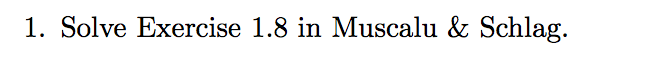
\includegraphics[width=0.5\textwidth]{HA-2-1.png}
\end{figure}
\end{question}

\begin{solution}
\end{solution}

\newpage

\begin{question}[2]
\hfill
\begin{figure}[h!]
  \centering
    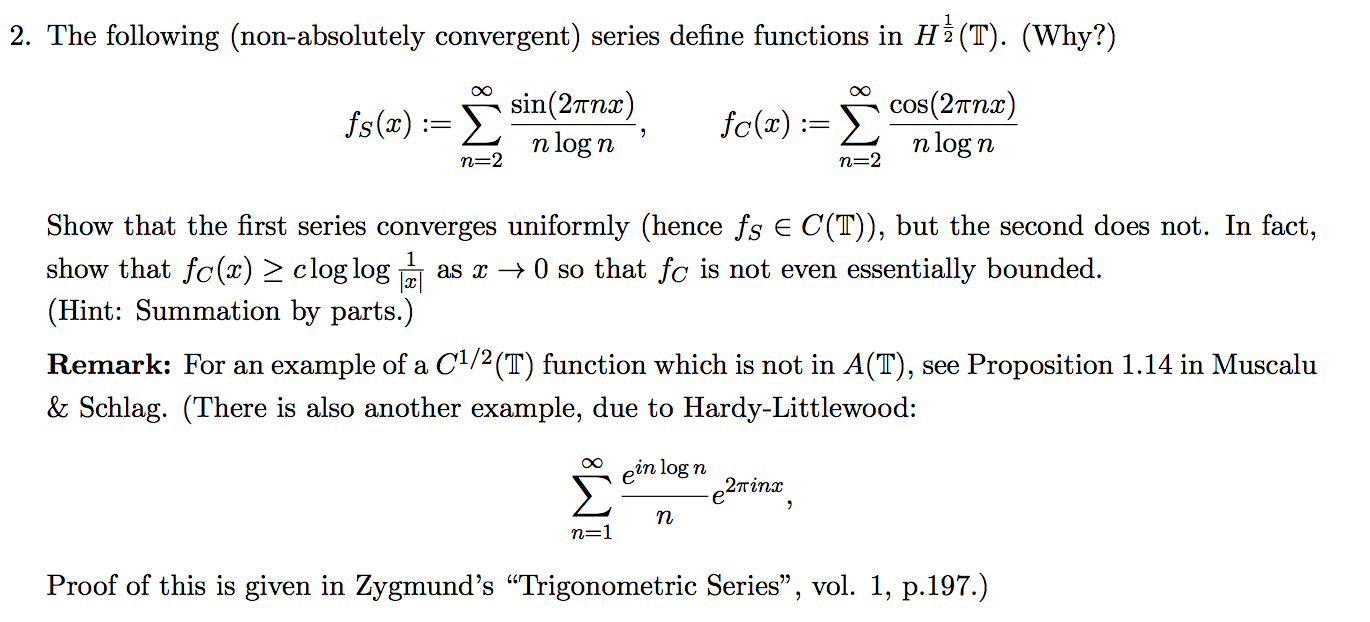
\includegraphics[width=1\textwidth]{HA-2-2.png}
\end{figure}
\end{question}
\begin{solution}
Define $g_{n,m} =
 \sum_{i = n}^{m} \dfrac{\sin(2\pi n x)}{n\log(n)}$. 
For $x \in [0,\dfrac{1}{m}]$, we have
\eQb
|g_{n,m}| &\leq& 
\sum_{i = n}^{m} \left| \dfrac{\sin(2\pi i x)}{i\log(i)} \right| 
\leq \sum_{i=n}^{m} \dfrac{2\pi i x}{i \log(i)} = \sum_{i=n}^{m} \dfrac{2 \pi x}{\log(i)} \\
&\leq& \dfrac{1}{\log(n)}  
\leq \dfrac{1}{m\log(n)} \sum_{i = n}^{m}{2\pi} \leq \dfrac{2\pi}{\log(n)}.  \\
\eQe
For $x \in [\dfrac{1}{m}, \dfrac{1}{n}]$, we obtain 

Therefore, we have that 
\eQb
|g_{n,m}| = O(\dfrac{1}{log(n)}),
\eQe
and the partial sums of $f_S$ is cauchy. Thus, $f_S$ converges uniformly and $f \in C(\mathbb{T})$.

\end{solution}

\newpage

\begin{question}[3]
\hfill
\begin{figure}[h!]
  \centering
    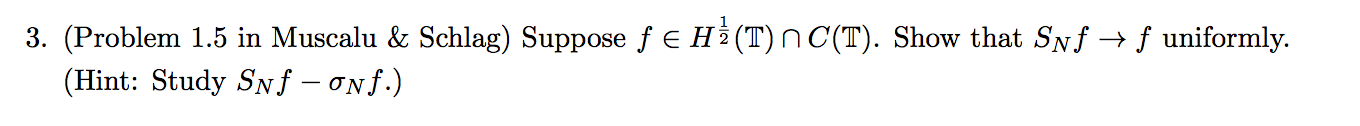
\includegraphics[width=1\textwidth]{HA-2-3.png}
\end{figure}
\end{question}
\begin{solution} 
By the triangle inequality of the supnorm, we have
\eQb
||S_N f - f ||_{\infty} \leq ||S_N f - \sigma_N f ||_{\infty} + 
||\sigma_N f - f||_{\infty},
\eQe
for all $N \in \mathbb{Z}^{+}$. As $f \in C(\mathbb{T})$, we have that 
$||\sigma_N f - f||_{\infty} \to 0$ as $N \to \infty$.
Therefore, 
it suffices to show that $||S_N f - \sigma_N f||_{\infty} \to 0$ as $N \to \infty$. 
By definition of $S_N$ and $\sigma_N$, triangle inequality, and Cauchy-Schwarz, we obtain 
\eQb
||S_N f - \sigma_N f||_{\infty} =  &\leq& \sum_{n = -N}^{N} \dfrac{|n|}{N}|\hat{f}(n)| \\
&\leq& \sum_{n=-M}^{M} \dfrac{|n||\hat{f}(n)|}{N} + (\sum_{N \geq |n| > M} \dfrac{|n|}{N^2})^{\frac{1}{2}}
(\sum_{N \geq |n| > M}|n||\hat{f}(n)|^2)^{\frac{1}{2}}, \\ 
&\leq& \sum_{n=-M}^{M} \dfrac{|n||\hat{f}(n)|}{N} + 
2(\sum_{N \geq |n| > M}|n||\hat{f}(n)|^2)^{\frac{1}{2}}, \\ 
\eQe
for any $N > M$. Taking $\limsup$ with respect to $N$ on both sides, we get
\eQb
\limsup_{N \to \infty} ||S_N f - \sigma_N f||_{\infty} &\leq&
2(\sum_{|n| > M}|n||\hat{f}(n)|^2)^{\frac{1}{2}}, \\ 
\eQe
for any $M$. As $f \in H^{\frac{1}{2}}(\mathbb{T})$, taking the limit as $M \to \infty$ gives
\eQb
\limsup_{N \to \infty} ||S_N f - \sigma_N f||_{\infty} &\leq& 0
\eQe
Hence, we have shown that $||S_N f - \sigma_N f||_{\infty} \to 0$ as $N \to \infty$ as desired. 
\hfill $\qed$
\end{solution}

\newpage

\begin{question}[4]
\hfill
\begin{figure}[h!]
  \centering
    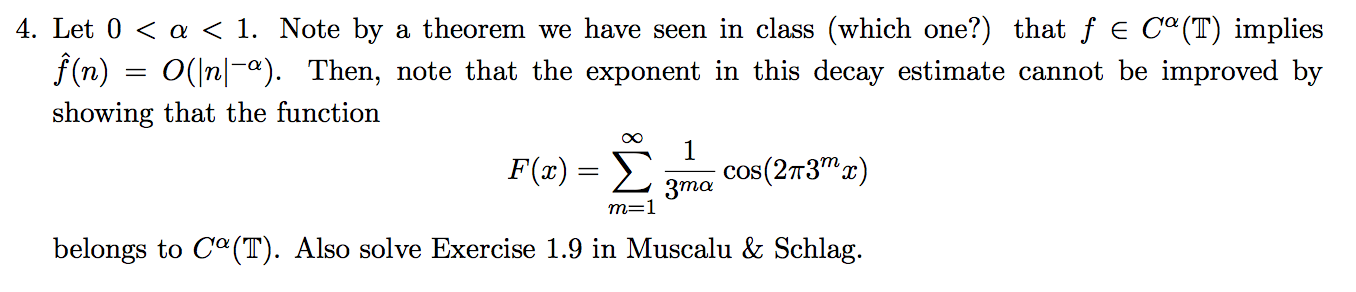
\includegraphics[width=1\textwidth]{HA-2-4.png}
\end{figure}
\end{question}
\begin{solution} \hfill \\
A theorem that gives this result of $f \in C^{\alpha}(\mathbb{T})
\implies \hat{f}(n) = O(n^{-\alpha})$ is recorded in section $1.4.4$, pg.18 of Schleg.

\bigskip

Now, we show that the exponent in the decay estimate
cannot be improved. We first show that $F \in 
C^{\alpha}(\mathbb{T})$. Fix $x,y \in \mathbb{T}$, such that $x \neq y$. Choose $K \in 
\mathbb{N}$ such that
$3^{-K-1} < |x - y| \leq 3^{-K}$. In particular, observe that, 
with this choice of $K$, we have $1 < 3^{K+1}|x-y| < 3$. 
It follows that
\eQb
\dfrac{|F(x) - F(y)|}{|x-y|^{\alpha}} &\leq& 
\sum_{m=1}^{K} \dfrac{|\cos(2\pi3^m x) - 
\cos(2\pi 3^m y)|}{3^{m\alpha} |x-y|^{\alpha}} +
\sum_{m=K+1}^{\infty} \dfrac{|\cos(2\pi3^m x) - 
\cos(2\pi 3^m y)|}{3^{m\alpha} |x-y|^{\alpha}} \\
&\leq& 
\sum_{m=1}^{K} \dfrac{2\pi3^m|x-y|}{3^{m\alpha} |x-y|^{\alpha}} +
\sum_{m=K+1}^{\infty} \dfrac{2}{3^{m\alpha} |x-y|^{\alpha}} \\
&=& 
2\pi \sum_{m=1}^{K} 
(3^{m}|x-y|)^{1-\alpha} 
+
\sum_{m=K+1}^{\infty} 2 
((3^{m}|x-y|)^{-\alpha} 
 \\  
&\leq& 
2\sum_{m=0}^{\infty} 3^{-\alpha m} \\ 
&\leq&
\dfrac{2}{1- 3^{-\alpha}} \\ 
\eQe 



\bigskip



 
\hfill $\qed$
\end{solution}

\newpage

\begin{question}[5]
\hfill
\begin{figure}[h!]
  \centering
    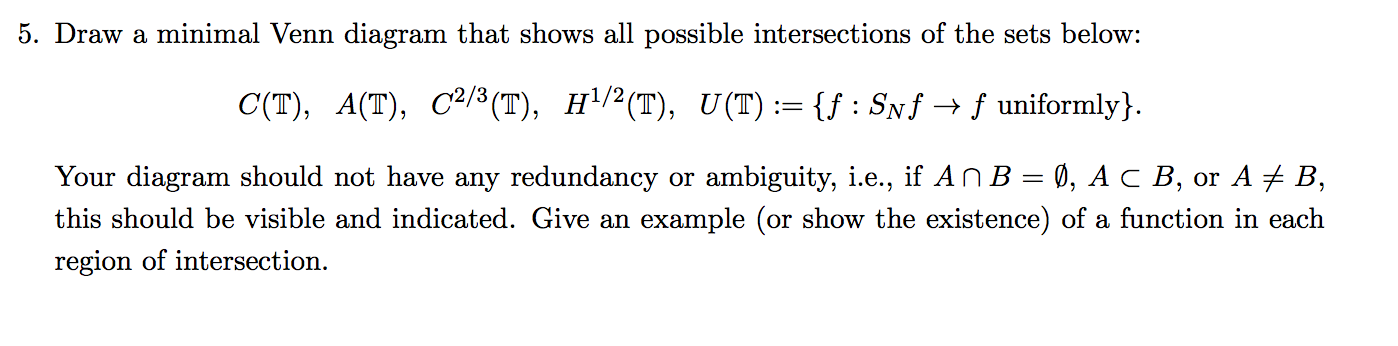
\includegraphics[width=1\textwidth]{HA-2-5.png}
\end{figure}
\end{question}
\begin{solution}
Since $S_n f $ is continuous, and uniform limit of a continuous function is continuous, we
have $U(\mathbb{T}) \subset C(\mathbb{T})$. We have previously shown that if $f \in A(\mathbb{T})$,
then $\{S_n f \}$ converges uniformly. This gives $A(\mathbb{T}) \subset U(\mathbb{T})$. As $\frac{2}{3}
> \frac{1}{2}$, the theorem $1.13$ from Schlag 
gives $C^{\frac{2}{3}}(\mathbb{T}) \subset H^{\frac{1}{2}}(\mathbb{T})$.


Now, from corollary $1.10$ from Schlag,
gives a function $g \in C(\mathbb{T})$ such that $g \not\in U(\mathbb{T})$. Hence,
$ C(\mathbb{T}) \setminus U(\mathbb{T}) \neq \emptyset$
 
In problem $2$, we have shown that $f_s \notin A(\mathbb{T})$, but $f_s \in U(\mathbb{T})$. Therefore,
$U(\mathbb{T}) \setminus A(\mathbb{T}) \neq \emptyset$. Now, take any $\dfrac{2}{3} >\alpha > \dfrac{1}{2}$,
and consider $F_{\alpha}$ from the problem $4$, parametrized by $\alpha$. It follows that $F_{\alpha}
\in A(\mathbb{T})$, and $F_{\alpha} \not\in C^{\frac{2}{3}}(\mathbb{T})$. Therefore, we have 
$A(\mathbb{T}) \setminus C^{\frac{2}{3}}(\mathbb{T}) \neq \emptyset$, and $F_{\frac{2}{3}} \in C^{\frac{2}{3}}
(\mathbb{T})$. Recapping the information we have
gathered so far gives the following figure:
\begin{figure}[!ht]
  \caption{Function spaces on $\mathbb{T}$}
  \centering
    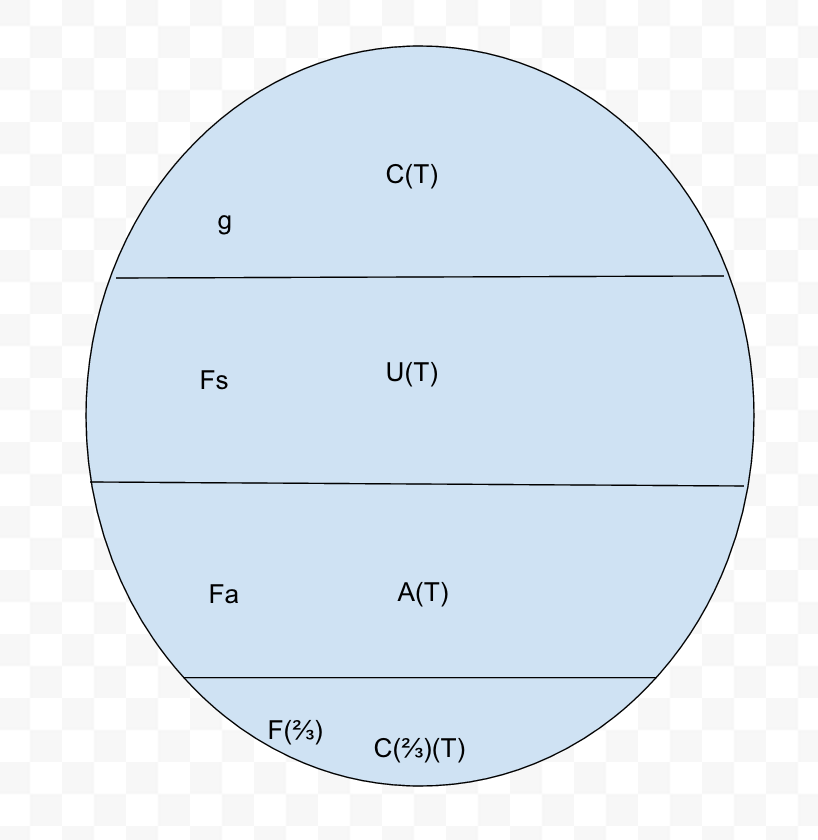
\includegraphics[width=0.5\textwidth]{fspace-1}
\end{figure}

Now, recall that $f_s$ from the problem $2$ is in $H^{\frac{1}{2}}(\mathbb{T})$, but not even essentially
bounded. Hence, $H^{\frac{1}{2}}(\mathbb{T}) \setminus C^{\frac{2}{3}}(\mathbb{T}) \neq \emptyset$. Now,
by the problem $3$, we have that $H^{\frac{1}{2}}(\mathbb{T}) \cap C(\mathbb{T}) \subset U(\mathbb{T})$,
and $f_s \in H^{\frac{1}{2}}(\mathbb{T}) \cap U(\mathbb{T})$. Recall that $F_{\alpha} \in H^{\frac{1}{2}}
(\mathbb{T})$. Hence, by preposition $1.14$ from there exists a function $h$ on $\mathbb{T}$ such that 

\newpage

$h \in U(\mathbb{T}) \setminus A(\mathbb{T})$ and $l \in A(\mathbb{T}) \setminus
C^{\frac{2}{3}}(\mathbb{T})$. Incorporating the additional information gives the following figure:

\begin{figure}[!ht]
  \caption{Function spaces on $\mathbb{T}$}
  \centering
    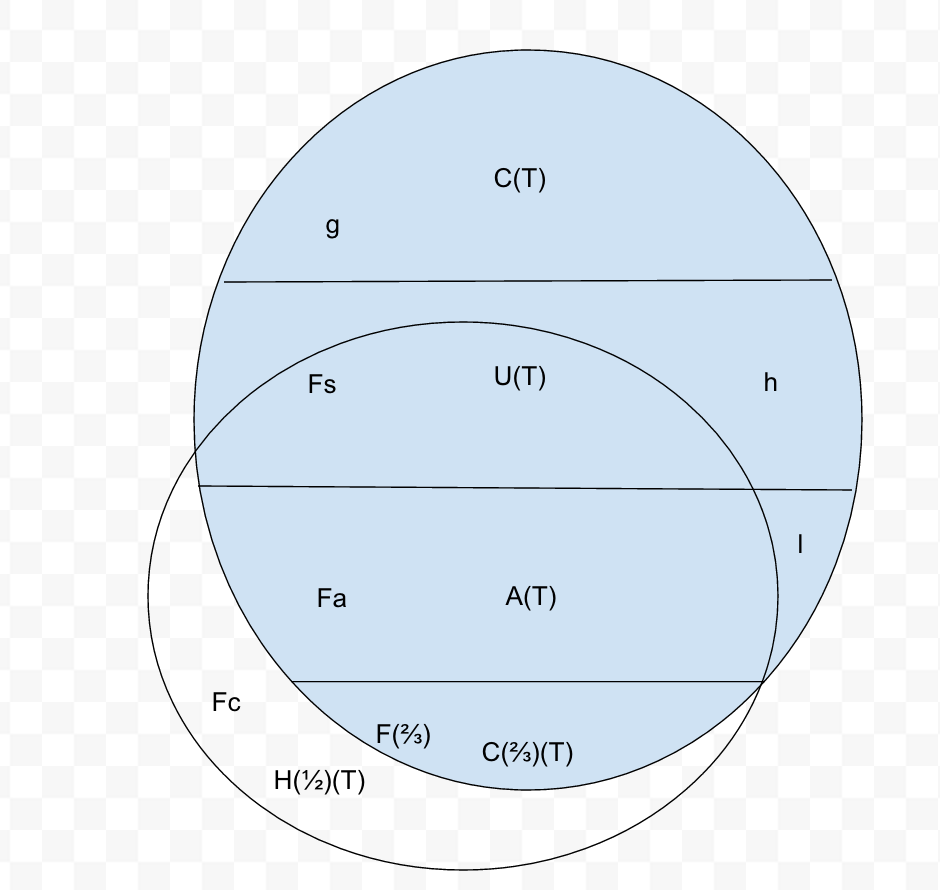
\includegraphics[width=0.5\textwidth]{fspace-2}
\end{figure}

This gives the adequate description of the function spaces on $\mathbb{T}$ for our interests.
\hfill $\qed$

\end{solution}

\bigskip

\end{document}
